%\subsection{Model Selection}
\subsection{Simulation: Estimator Selection}
An applied researcher has to make certain assumptions on the data at hand for the validity of the method used for causal identification. The trade off she faces is to use a general method without putting restrictive assumptions on the data or to use a parsimonious method if she can justify the data satisfies the relevant assumptions. If the causal identification assumption of the method fails, then the estimates will be biased and uninterpretable. On the other hand, the more general the model is, the more imprecise estimates become.
A common way to show the validity of a method is to run multiple regression specifications and to compare the results given the intuition on the causal links and economic theory. Nevertheless, these are based on a single sample.
Multiple samples can be simulated by a DGP adapted to the real world data and assuming the causal identification assumptions hold to see the finite sample properties of the methods in question.

The DGP described in the previous subsection is well-adapted to a GFE setting with two groups. The unobserved heterogeneity has two distinct time patterns. Table 1 reports on finite sample properties of pooled OLS, FE, TWFE, IFE estimators. They are compared in terms of bias, variance and coverage probability.
It is important to note that $\alpha_1^0$ and $\alpha_2^0$ are functions of t. In return, their impact on the outcome and the regressors increase over time.  The impact of $\alpha$ on regressor $X_2$ is nonlinear and small\footnote{Due to the fact that it is scaled by 0.05 in order to avoid an out of proportion contribution to the regressor when T=20.} in the initial periods but grows fast overtime. While the impact of $\alpha$ on regressor $X_1$ is linearly increasing overtime. This impact determines the omitted variable bias in small samples when the they are not accounted for. Pooled OLS estimator suffers from large biases, FE and TWFE perform relatively well with small bias and the coverage probability around 95 percent when T and N are small. However, as either T or N increases the bias increases, the coverage probability gets smaller such that the true value is never in the confidence intervals suggesting the variance decreases while driven by the bias the root mean square error stays relatively high. IFE model is estimated with r=2 factors. IFE estimates have a quite small bias and relatively high RMSE driven by the estimator variance throughout. This suggests that IFE estimates suffer from overfitting in this setup. As a result the coverage probability stays below 95 percent.
As the magnitude of $\alpha$ increase, GFE estimates perform better. They have low bias and low variance for all T and N and the coverage probability converges to 95 percent level at T=10,  N=100. 
\paragraph{Consistency and the asymptotic normality of $\hat{\alpha}$.} %or is it asymptotic dist?
IFE, TWFE
%\footnote{Apart from the DD.}
, FE treat the unobserved effects as nuisance parameter. They are not reported nor interpreted. GFE claims that the grouped-fixed effects are consistently estimated when both N,T $\to \infty$. %Note: could they account for DD?
Figure \ref{fig:alpha11}\footnote{The remaining grouped-fixed effect estimates are omitted in the paper since all shows a similar pattern. All GFE estimates from the simulations in this paper can be found in github.com/baharcos/gfe.} shows that $\alpha_{11}$ estimates are biased\footnote{It should be noted that I do not calculate an intercept in my implementation of the GFE estimator where I get the estimates. Even though $\upsilon_{it}$ are i.i.d. standard normal, they might have some mean when sampled, particularly in small samples. This, combined with the small value of $\alpha_{11}^0 = 1.05$ might have caused this bias. However, I cannot verify it for the time being.} when T=5, N=50 but they recover quickly when either T or N increases. They are normally distributed and tails of the normal distribution gets thinner in either direction. This result enables statistical inference of $\hat{\alpha}$ when the number of groups are correctly specified. % Note: is this the way to say it. showing consistency in finite sample? 


% where the [p] is is [h!] means herebut it does not put it there sometimes it does not work because it thinks its very dumb. you can go for  a floatbreak to force it.

%\usepackage{placeins} %use that package
\begin{table}[p]
    \centering
    %\scalebox{0.9}{
    \caption{Simulation: Bias, RMSE and CP of estimators in the presence of grouped patterns of unobserved heterogeneity.}
    \begin{tabular}{lll|ccc|ccc}
\toprule
%&      &        &  \multicolumn{3}{|c|}{$\hat{\theta_1}$} & \multicolumn{3}{|c|}{$\hat{\theta_2}$} \\
   &      &        &              &  $\hat{\theta_1}$   &                &    & $\hat{\theta_2}$ & \\
   %\cline{4-6} \cline{6-9} %\hline
T & N & Estimator &      Bias     &      RMSE     &   CP      &      Bias     &      RMSE     &   CP      \\
\midrule
5  & 50   & OLS  &  0.054102 &  0.074713 &                 0.798 &  0.016240 &  0.051727 &                 0.924 \\
   &      & FE  &  0.002876 &  0.043734 &                 0.930 &  0.001944 &  0.042465 &                 0.937 \\
   &      & TWFE  &  0.002372 &  0.043964 &                 0.959 &  0.001864 &  0.042802 &                 0.959 \\
   &      & IFE &  -0.000581 &  0.053420 &                 0.796 &  0.002265 &  0.051574 &                 0.805 \\
   &      & GFE  &  0.002966 &  0.039885 &                 0.913 & -0.000647 &  0.039435 &                 0.924 \\
    %\hline
   & 100  & OLS  &  0.054161 &  0.065063 &                 0.654 &  0.015829 &  0.036894 &                 0.940 \\
   &      & FE  &  0.004010 &  0.031767 &                 0.928 &  0.000860 &  0.029627 &                 0.944 \\
   &      & TWFE  &  0.003267 &  0.031742 &                 0.954 &  0.001018 &  0.029656 &                 0.971 \\
   &      & IFE  &  0.000032 &  0.037603 &                 0.789 &  -0.001096 &  0.035950 &                 0.824 \\
   &      & GFE  &  0.002530 &  0.028159 &                 0.923 & -0.000581 &  0.026704 &                 0.945 \\
   %\hline
   & 1000 & OLS  &  0.054668 &  0.055754 &                 0.001 &  0.015190 &  0.018635 &                 0.714 \\
   &      & FE  &  0.004058 &  0.010395 &                 0.920 &  0.000954 &  0.009640 &                 0.949 \\
   &      & TWFE  &  0.003208 &  0.010058 &                 0.953 &  0.000937 &  0.009642 &                 0.972 \\
   &      & IFE   &  0.000724 &  0.010579 &                 0.865 & -0.000413 &  0.011016 &                 0.849 \\
   &      & GFE  &  0.002218 &  0.008892 &                 0.921 &  0.000372 &  0.008639 &                 0.932 \\
   %\hline
10 & 50   & OLS  &  0.105636 &  0.113233 &                 0.276 &  0.060948 &  0.073050 &                 0.694 \\
   &      & FE  &  0.012663 &  0.032757 &                 0.913 &  0.014366 &  0.032955 &                 0.919 \\
   &      & TWFE  &  0.010175 &  0.032108 &                 0.933 &  0.012137 &  0.032050 &                 0.938 \\
   &      & IFE  & -0.000596 &  0.031605 &                 0.878 & -0.000970 &  0.030777 &                 0.890 \\
   &      & GFE  & -0.000390 &  0.027524 &                 0.929 & -0.000520 &  0.025941 &                 0.955 \\
  %\hline
   & 100  & OLS  &  0.107757 &  0.111319 &                 0.039 &  0.062267 &  0.068259 &                 0.441 \\
   &      & FE  &  0.014326 &  0.025154 &                 0.894 &  0.014199 &  0.024524 &                 0.902 \\
   &      & TWFE  &  0.011853 &  0.023765 &                 0.930 &  0.012174 &  0.023278 &                 0.935 \\
   &      & IFE   &  0.000574 &  0.020085 &                 0.918 &  0.000278 &  0.020533 &                 0.920 \\
   &      & GFE  &  0.000420 &  0.017785 &                 0.954 &  0.000179 &  0.017274 &                 0.958 \\
   %\hline
   & 1000 & OLS  &  0.107998 &  0.108382 &                 0.000 &  0.061307 &  0.061987 &                 0.000 \\
   &      & FE  &  0.013653 &  0.015149 &                 0.458 &  0.014833 &  0.016210 &                 0.392 \\
   &      & TWFE  &  0.010977 &  0.012729 &                 0.644 &  0.012444 &  0.013996 &                 0.564 \\
   &      & IFE  &  0.000215 &  0.006599 &                 0.906 &  0.000244 &  0.006239 &                 0.926 \\
   &      & GFE  &  0.000307 &  0.005713 &                 0.955 &  0.000282 &  0.005541 &                 0.955 \\
    %\hline
20 & 50   & OLS  &  0.237060 &  0.239771 &                 0.000 &  0.434061 &  0.434975 &                 0.000    \\
   &       & FE  &  0.048879 &  0.054307 &                 0.477 &  0.173001 &  0.174211 &                 0.000 \\
   &      & TWFE  &  0.044322 &  0.050241 &                 0.558 &  0.151598 &  0.153061 &                 0.000 \\
   &      & IFE   &  0.000915 &  0.019849 &                 0.912 &  0.000100 &  0.019723 &                 0.919 \\
   &      & GFE  &  0.000512 &  0.017937 &                 0.957 &  0.000251 &  0.017497 &                 0.959 \\
    %\hline
   & 100  & OLS  &  0.236169 &  0.237680 &                 0.000 &  0.432264 &  0.432755 &                 0.000 \\
   &      & FE  &  0.047993 &  0.051000 &                 0.205 &  0.172927 &  0.173593 &                 0.000 \\
   &      & TWFE  &  0.042917 &  0.046133 &                 0.292 &  0.150358 &  0.151148 &                 0.000 \\
   &      & IFE    &  0.000654 &  0.014032 &                 0.922 & -0.000159 &  0.014385 &                 0.913 \\
   &      & GFE  &  0.000265 &  0.013012 &                 0.946 &  0.000533 &  0.013551 &                 0.932 \\
   %\hline
   & 1000 & OLS  &  0.236499 &  0.236630 &                 0.000 &  0.433180 &  0.433221 &                 0.000 \\
   &      & FE  &  0.047854 &  0.048164 &                 0.000 &  0.172728 &  0.172784 &                 0.000 \\
   &      & TWFE  &  0.042512 &  0.042839 &                 0.000 &  0.148935 &  0.149002 &                 0.000 \\
   &      & IFE    &  0.000205 &  0.004213 &                0.949 & -0.000645 &  0.004171 &                 0.948 \\
   &      & GFE  &  0.000160 &  0.003963 &                 0.954 &  0.000003 &  0.003857 &                 0.962 \\
\bottomrule
\end{tabular}

    %}
    \label{tab:table0}
\end{table}
%\FloatBarrier %floatbarrier will enforce it to be at most here. like nothing that is below the float barrier can be above smtht hat is above the float barrier

\begin{figure}[h]
\centering
\includegraphics[scale=0.25]{figures/samplingalpha1.png}
\caption{Sampling distribution of $\hat{\alpha}_{11}$ where $G = G^0 = 2$ and R=1000 simulation runs.}
\label{fig:alpha11}
\end{figure}


\subsection{Simulation: Number of Groups}
%\subsubsection{} I can make subsections heuristics, estimating number of groups, sampling distribution maybe after the consistent comment.
In the GFE model, \textcite{bonhomme2015grouped} assumes the true number of groups is known by the researcher. However, the number of groups is %often
estimated even when it is based on economic theory. In applications, this estimation is based on the single sample the researcher observes and she can easily  misspecify the number of groups. This subsection studies the number of group selection and the finite sample properties of GFE estimates of $\theta$ when the number of groups is misspecified at G = 1, 3, 4.

A researcher could employ an information criterion to specify the number of groups from regression runs with different specifications. The information criterion balances a penalty for overspecification and m
Based on \textcite{bai2002determining} \textcite{bonhomme2015grouped} suggests the following bayesian information criterion (BIC) for estimating $G^0$ consistently:
\begin{align}
    BIC(G) = \dfrac{1}{N} \sumi \sumt \left(y_{it} - x_{it}'\hat{\theta}^(G) - \hat{\alpha}_{g_it}^(G) \right)^2 + \hat{\sigma}^2 \dfrac{GT + N + K}{NT}ln(NT),
\end{align}
where $\hat{\sigma}^2$ is a consistent estimate of the variance of the error terms. To do so requires N and T to grow at the same rate. Table \ref{tab:tablebic} reports on the selection rate of the number of groups using the simulation results of GFE estimator with different number of groups. The maximum number of groups is set to 4. The BIC provided estimates the true number of groups only when $T=20, N=50$ as expected. In every other case it tends to over-select. This suggests two things: First, the penalty term of the criterion needs to be adapted for small T large N. Such a BIC was developed in \textcite{janys2021mental}, however they report it turns out to be too steep. Second, the over-selection could occur because the efficiency cost of over-specifying is relatively low. 

\begin{table}[h!]
    \centering
    \caption{Simulation: Selecting Number of Groups by BIC}
    \begin{tabular}{llrrrr}
\toprule
%   &      &   &  Selection rate && \\
T & N & G=1 & G=2 & G=3 & G=4                \\
\midrule
5  & 50    &           0. &           0. &           0.075 &           0.925 \\
   & 100   &           0. &           0. &           0.003 &           0.997 \\
   & 1000  &           0. &           0. &           0.000 &           1.000 \\
10 & 50    &           0. &           0. &           0.196 &           0.395 \\
   & 100   &           0. &           0. &           0.056 &           0.943 \\
   & 1000  &           0. &           0. &           0.000 &           1.000 \\
20 & 50    &           0. &           1. &           0.000 &           0.000 \\
   & 100   &           0. &           0. &           0.006 &           0.000 \\
   & 1000  &           0. &           0. &           0.000 &           1.000 \\
\bottomrule
\end{tabular}

    \label{tab:tablebic}
\end{table}


An under-specification of the number of groups is unable to account for the group structure; therefore it suffers from the omitted variable bias. Any group specification $G \geq G^0$, however accounts for the group structure, and its estimate of $\theta$ is consistent under assumption $\mathcal{A}$. As the proof of the theorem \ref{eqn:gfeconsist} for $\hat{\theta}$ does not depend on G. See appendix A of \textcite{bonhomme2015grouped}.

Figure \ref{fig:gs} aims to show the consistency of the GFE estimates of $\theta_1$ and Figure \ref{fig:gsn} aims to show the consistency of the GFE estimates of $\theta_2$.
The last row shows the estimator with G=1 is biased and inconsistent while G=2,3,4, where $G^0=2$ are consistent.
Linear or nonlinear nature of the correlation between the regressors and the grouped-fixed effect does not seem to affect this result.
%The last row again shows the estimates of G=1 is biased and inconsistent. While G=2,3,4, where $G^0=2$ is consistent.

%which its corresponding regressor is linearly correlated with the grouped-fixed effects. which its corresponding regressor is nonlinearly correlated with the grouped-fixed effects

\begin{figure}[p]
\begin{flushleft}
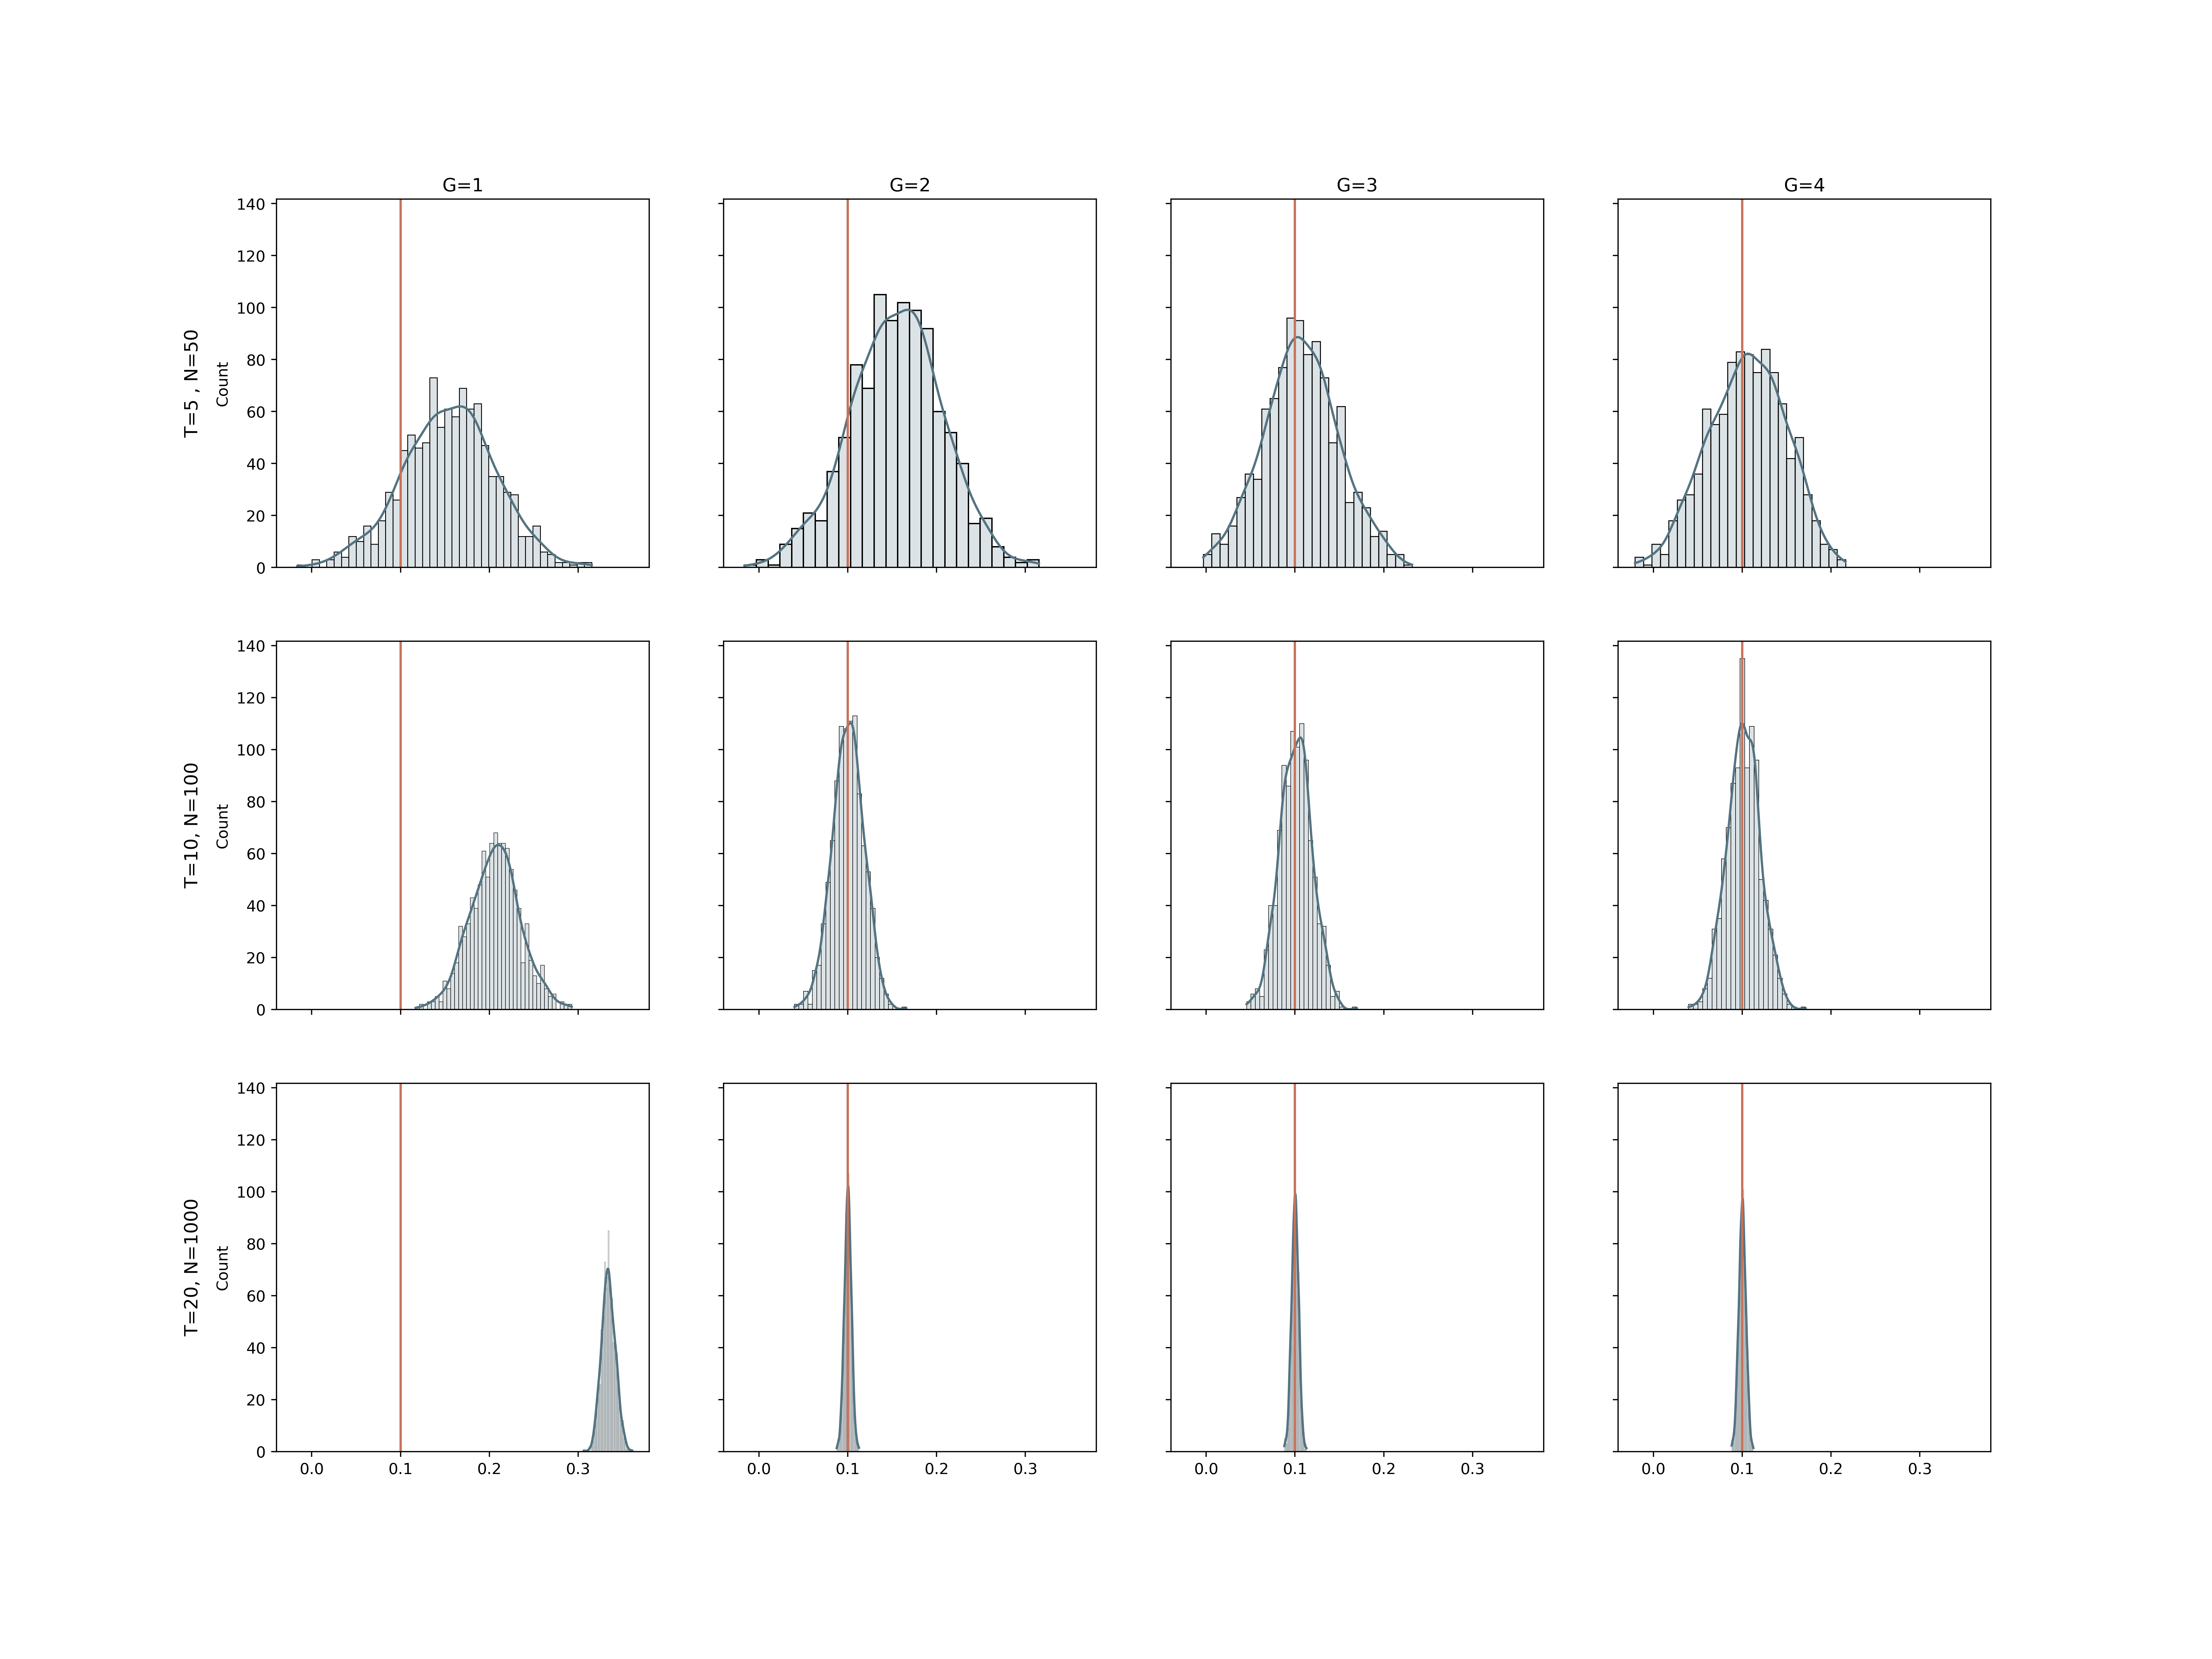
\includegraphics[scale=0.31]{figures/groupssamplingplot1.png}
\end{flushleft}
\caption{Sampling Distribution of $\hat{\theta_1}$ when both T and N increases in different number of group specifications where $G^0 = 2$.}
\label{fig:gs}
\end{figure}

Figure \ref{fig:gsn} is aimed to show the consistency of the GFE estimates of $\theta_2$ which its corresponding regressor is nonlinearly correlated with the grouped-fixed effects. The sampling distribution when both T and N increases. The last row again shows the estimates of G=1 is biased and inconsistent. While G=2,3,4, where $G^0=2$ is consistent.

\begin{figure}[h]
\begin{flushleft}
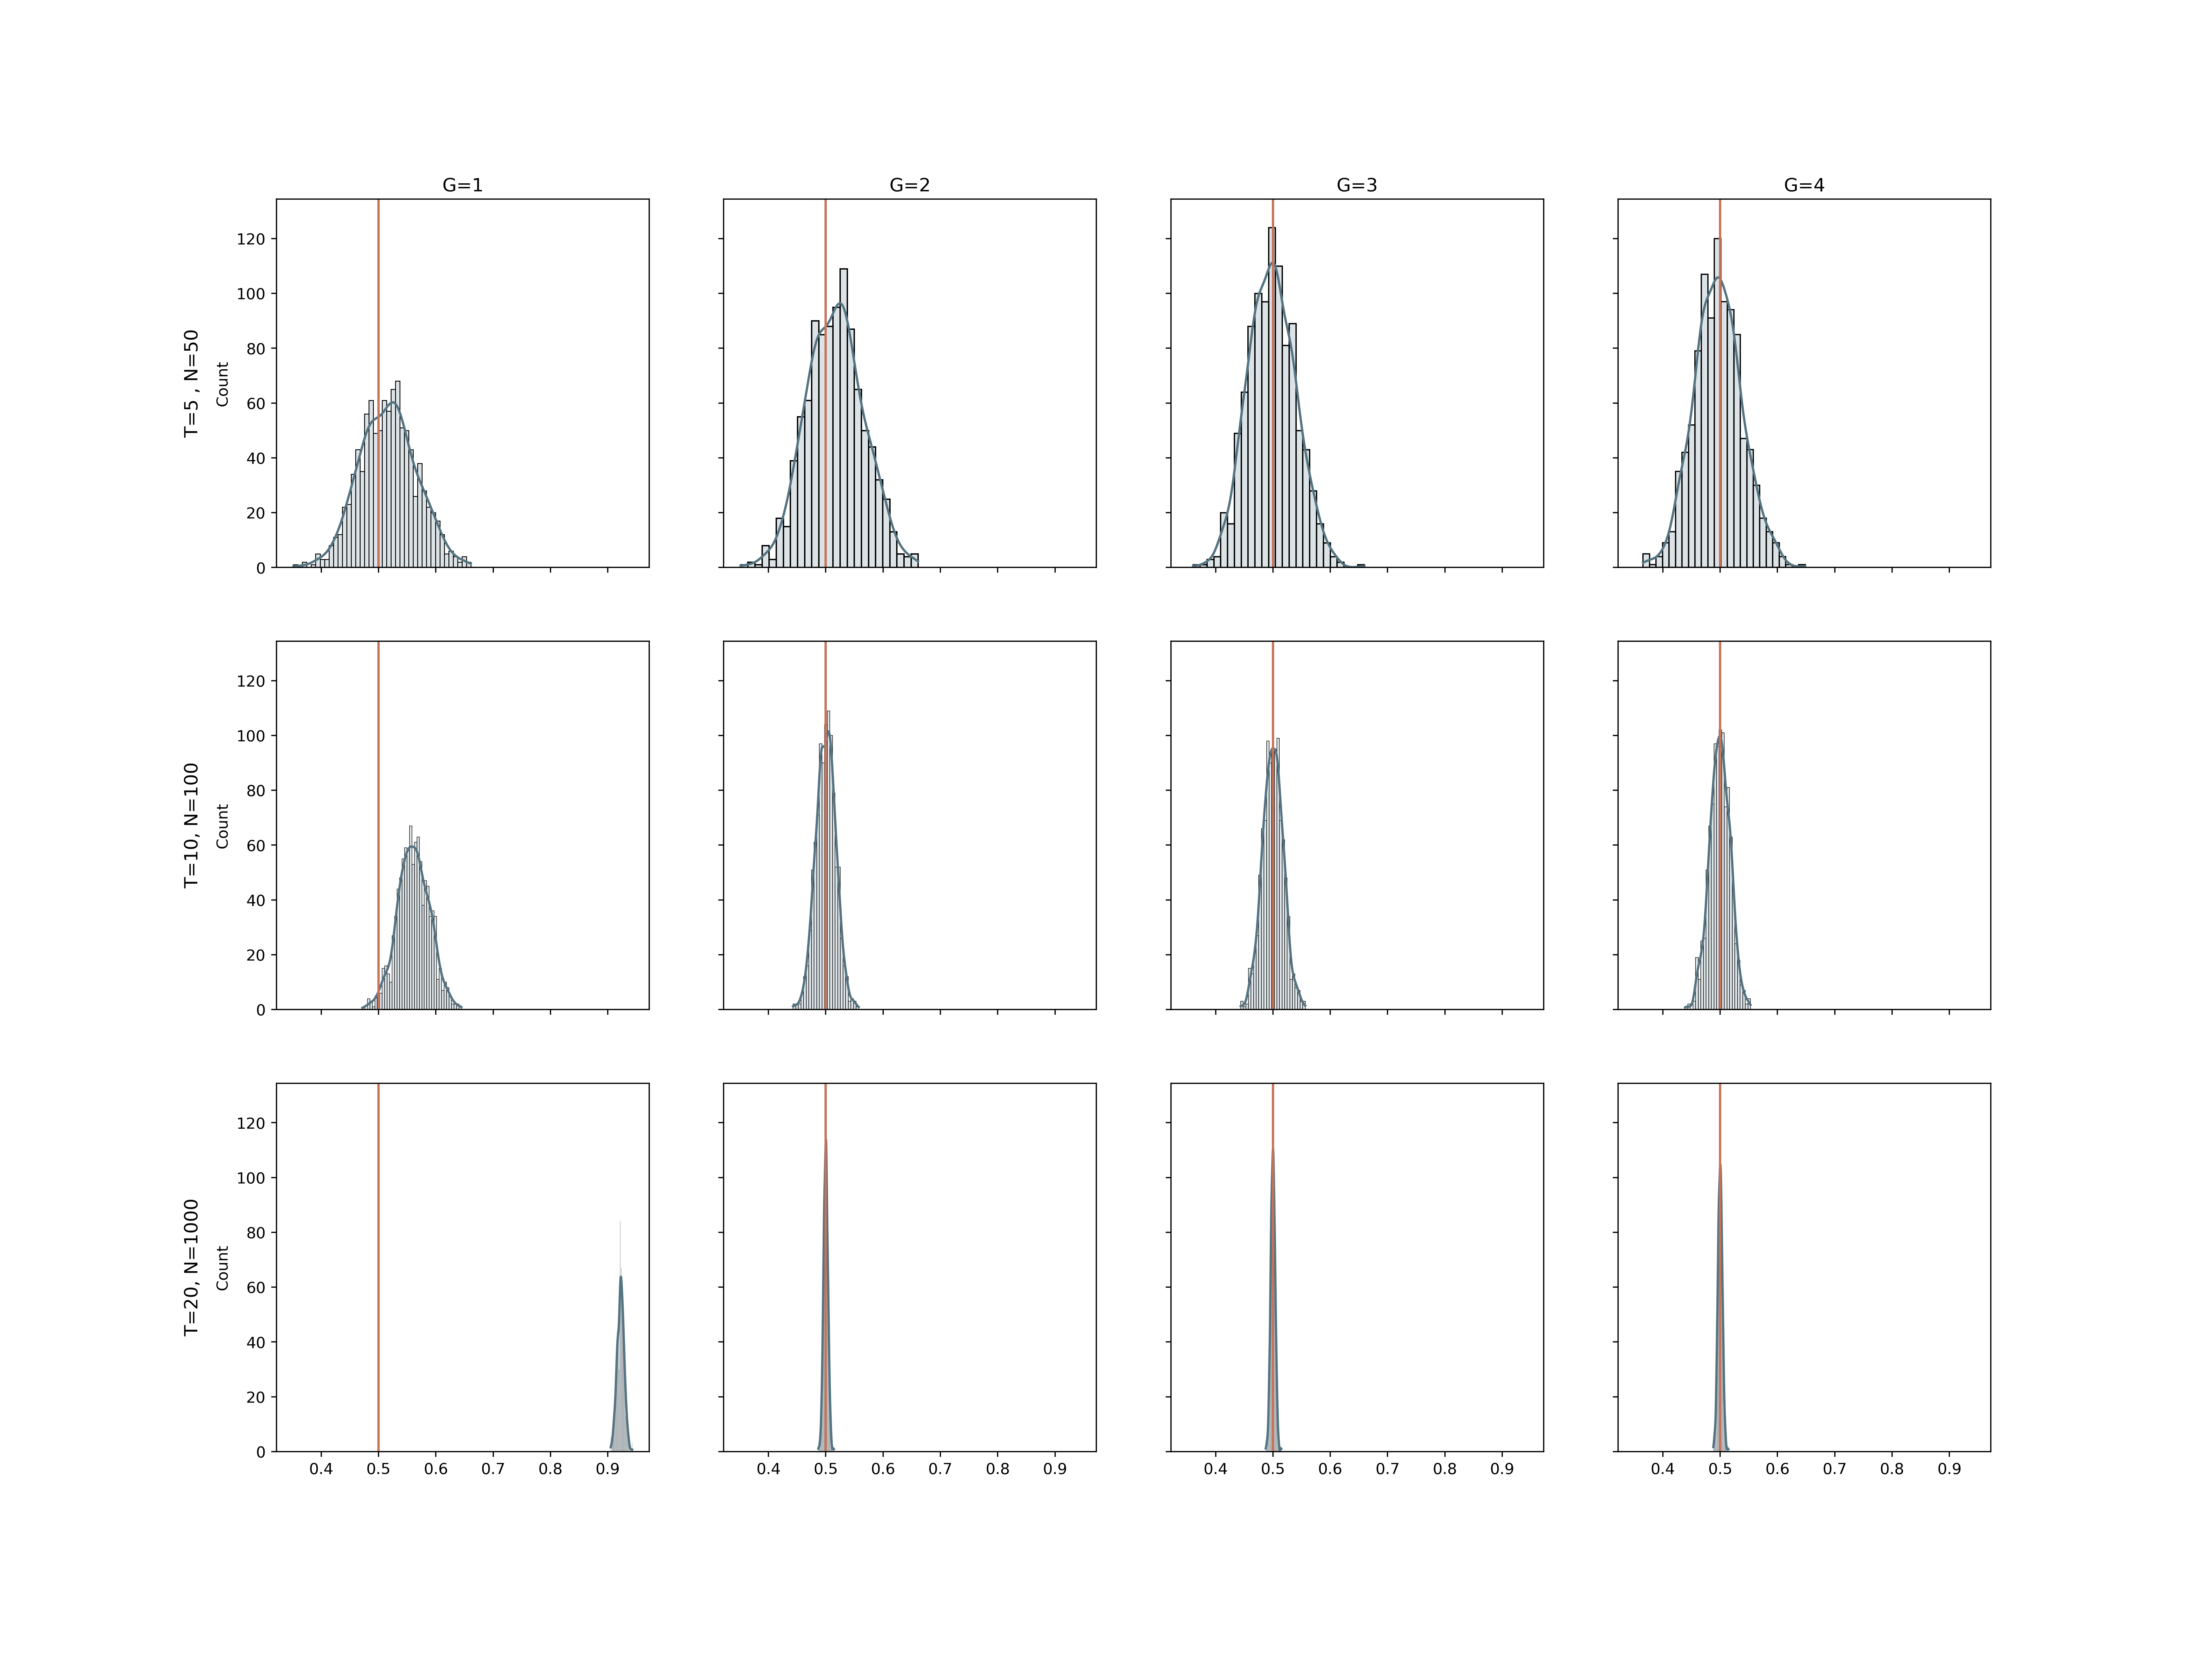
\includegraphics[scale=0.31]{figures/groupssamplingplot.png}
\end{flushleft}
\caption{Sampling Distribution of $\hat{\theta_2}$ when both T and N increases in different number of group specifications where $G^0 = 2$.}
\label{fig:gsn}
\end{figure}

Intuition from OLS suggests that including an irrelevant regressor do not effect the asymptotic properties of the estimator. Nevertheless, some finite sample inefficiency is expected. Before looking at the finite sample properties of the GFE estimator where the number groups are misspecified, we look at how the individuals are divided into groups and how the additional $\hat{\alpha}$ are estimated for some intuition.

Figure \ref{fig:staringalphas} shows the starting value of $\alpha$ for specified number of groups of G=1,2,3,4. For G=2, the true value of $\alpha$ is used as the starting value in Figure \ref{fig:staringalphas}.

\begin{figure}[h!]
\centering
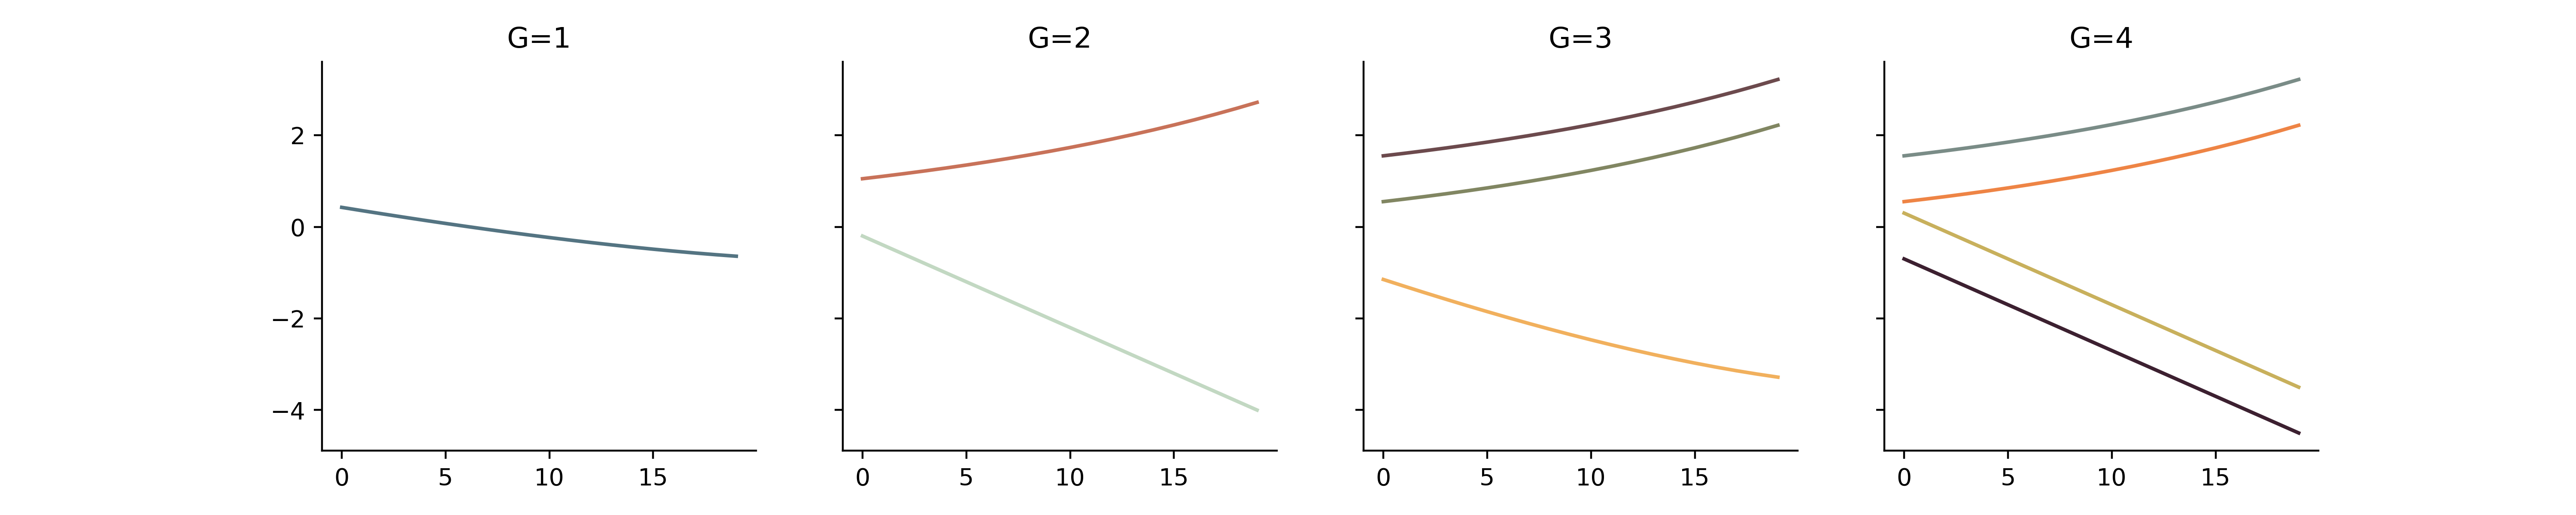
\includegraphics[scale=0.4]{figures/startingvalues.png}
\caption{$\alpha^{(0)}$ in Algorithm 1}
\label{fig:staringalphas}
\end{figure}

Specification $G=1$ basically introduces time dummies into the regression and does not account for the group structure leading to an omitted variable bias. We can think of it as as allowing only for $\xi_t$ and assuming $c_i, \lambda_i' f_t, \alpha_{gt} = 0$ in the context of the theoretical background. 
To contrasts, specification $G=2$ shows and accounts for the grouped patterns of heterogeneity in the data. Specification $G=3$ and $G=4$ divides the groups into subgroups and fits group heterogeneity with parts of idiosyncratic error term. They introduce additional group-time dummies into the regression. The added fit of over specified groups comes from the idiosyncratic error term that is irrelevant for the causal effect. However, the $\hat{\alpha}_{G>G^0}$ estimates added by number of group overspecification account for both the grouped patterns of heterogeneity and the idiosyncratic error as the individuals divided into more groups. When the number of groups are overspecified inference is not possible for $\hat{\alpha}_{G>G^0}$. Relating to Remark 4 in \textcite{bai2009panel} on p. 1247, some efficiency loss is expected.

Table \ref{tab:table2} reports on bias, RMSE and CP of the GFE estimator with different number of groups specifications. The results show that $G \leq G^0$ is inadequate. On the other hand when $G \ge G^0$, the coverage probabilities stays comparable and close to $G = G^0$. Unlike IFE in \ref{tab:table0} where the overfitting decreased the bias and increased the variance. The bias and RMSE of $G \ge G^0$ is remains similar with minor differences to $G = G^0$ for each N and T suggesting a similarity in their asymptotic distribution. 

\begin{table}[p]
    \centering
    \begin{tabular}{lll|ccc|ccc}
\toprule
   &      &   &       &  $\hat{\theta_1}$   &             &    & $\hat{\theta_2}$ & \\
   \hline
T & N & G & Bias &    RMSE       &      CP     &    Bias &    RMSE       &      CP           \\
\midrule
5  & 50   & 1 &  0.054515 &  0.075302 &                 0.774 & 0.016464 &  0.052199 &                 0.924 \\
   &      & 2 &  0.054515 &  0.075302 &                 0.609 & 0.016464 &  0.052199 &                 0.817 \\
   &      & 3 &  0.007147 &  0.042757 &                 0.874 &-0.001957 &  0.041414 &                 0.895 \\
   &      & 4 &  0.005630 &  0.043443 &                 0.852 &-0.003852 &  0.042086 &                 0.864 \\
   & 100  & 1 &  0.053953 &  0.065008 &                 0.639 & 0.016095 &  0.037208 &                 0.938 \\
   &      & 2 &  0.002530 &  0.028159 &                 0.923 &-0.000581 &  0.026704 &                 0.945 \\
   &      & 3 &  0.005137 &  0.031111 &                 0.880 &-0.001322 &  0.028468 &                 0.907 \\
   &      & 4 &  0.004068 &  0.030487 &                 0.864 &-0.002602 &  0.029530 &                 0.880 \\
   & 1000 & 1 &  0.054041 &  0.055140 &                 0.001 & 0.015190 &  0.018637 &                 0.713 \\
   &      & 2 &  0.002218 &  0.008892 &                 0.921 & 0.000372 &  0.008639 &                 0.932 \\
   &      & 3 &  0.004243 &  0.010095 &                 0.865 & 0.000682 &  0.009194 &                 0.909 \\
   &      & 4 &  0.002963 &  0.009841 &                 0.870 & 0.000414 &  0.009327 &                 0.896 \\
10 & 50   & 1 &  0.105206 &  0.112956 &                 0.264 & 0.059915 &  0.072625 &                 0.686 \\
   &      & 2 & -0.000390 &  0.027524 &                 0.929 &-0.000520 &  0.025941 &                 0.955 \\
   &      & 3 &  0.000526 &  0.028568 &                 0.910 &-0.001678 &  0.026467 &                 0.945 \\
   &      & 4 &  0.002240 &  0.029164 &                 0.903 &-0.002827 &  0.027290 &                 0.917 \\
   & 100  & 1 &  0.106493 &  0.110116 &                 0.038 & 0.060961 &  0.067022 &                 0.455 \\
   &      & 2 &  0.000420 &  0.017785 &                 0.954 & 0.000179 &  0.017274 &                 0.958 \\
   &      & 3 &  0.001118 &  0.018308 &                 0.941 &-0.000121 &  0.018026 &                 0.941 \\
   &      & 4 &  0.001640 &  0.018908 &                 0.924 &-0.000780 &  0.017871 &                 0.940 \\
   & 1000 & 1 &  0.105803 &  0.106192 &                 0.000 & 0.059296 &  0.059985 &                 0.000 \\
   &      & 2 &  0.000307 &  0.005713 &                 0.955 & 0.000282 &  0.005541 &                 0.955 \\
   &      & 3 &  0.000304 &  0.005857 &                 0.950 & 0.000269 &  0.005664 &                 0.946 \\
   &      & 4 &  0.000339 &  0.005970 &                 0.934 & 0.000150 &  0.005745 &                 0.938 \\
20 & 50   & 1 &  0.238163 &  0.240944 &                 0.000 & 0.429078 &  0.430069 &                 0.000 \\
   &      & 2 &  0.000512 &  0.017937 &                 0.957 & 0.000251 &  0.017497 &                 0.959 \\
   &      & 3 &  0.001167 &  0.018181 &                 0.942 &-0.000483 &  0.017839 &                 0.949 \\
   &      & 4 &  0.001947 &  0.018758 &                 0.939 &-0.001245 &  0.018226 &                 0.944 \\
   & 100  & 1 &  0.235297 &  0.236822 &                 0.000 & 0.424235 &  0.424768 &                 0.000 \\
   &      & 2 &  0.000265 &  0.013012 &                 0.946 & 0.000533 &  0.013551 &                 0.932 \\
   &      & 3 &  0.000630 &  0.013289 &                 0.945 & 0.000072 &  0.013842 &                 0.929 \\
   &      & 4 &  0.001156 &  0.013439 &                 0.935 &-0.000434 &  0.014113 &                 0.921 \\
   & 1000 & 1 &  0.234128 &  0.234257 &                 0.000 & 0.422433 &  0.422477 &                 0.000 \\
   &      & 2 &  0.000160 &  0.003963 &                 0.954 & 0.000003 &  0.003857 &                 0.962 \\
   &      & 3 &  0.000167 &  0.004001 &                 0.951 & 0.000003 &  0.003884 &                 0.964 \\
   &      & 4 &  0.000193 &  0.004069 &                 0.943 &-0.000039 &  0.003911 &                 0.955 \\
\bottomrule
\end{tabular}

    \caption{Simulation: GFE Group Specification} %subject to change
    \label{tab:table2}
\end{table}

Figure \ref{fig:cilength} shows the average confidence intervals of the GFE estimators with different number of groups specifications for $\theta_1 = 0.10$. The average is taken over 1000 replications when T=10, N=100. The horizontal blue dotted line marks the true, black dots are the mean of the $\theta_1$ estimates for the given estimator with the number of groups specification stated in x-axis. The confidence intervals overlap when $G \geq G^0$. 
\begin{figure}[h]
\centering
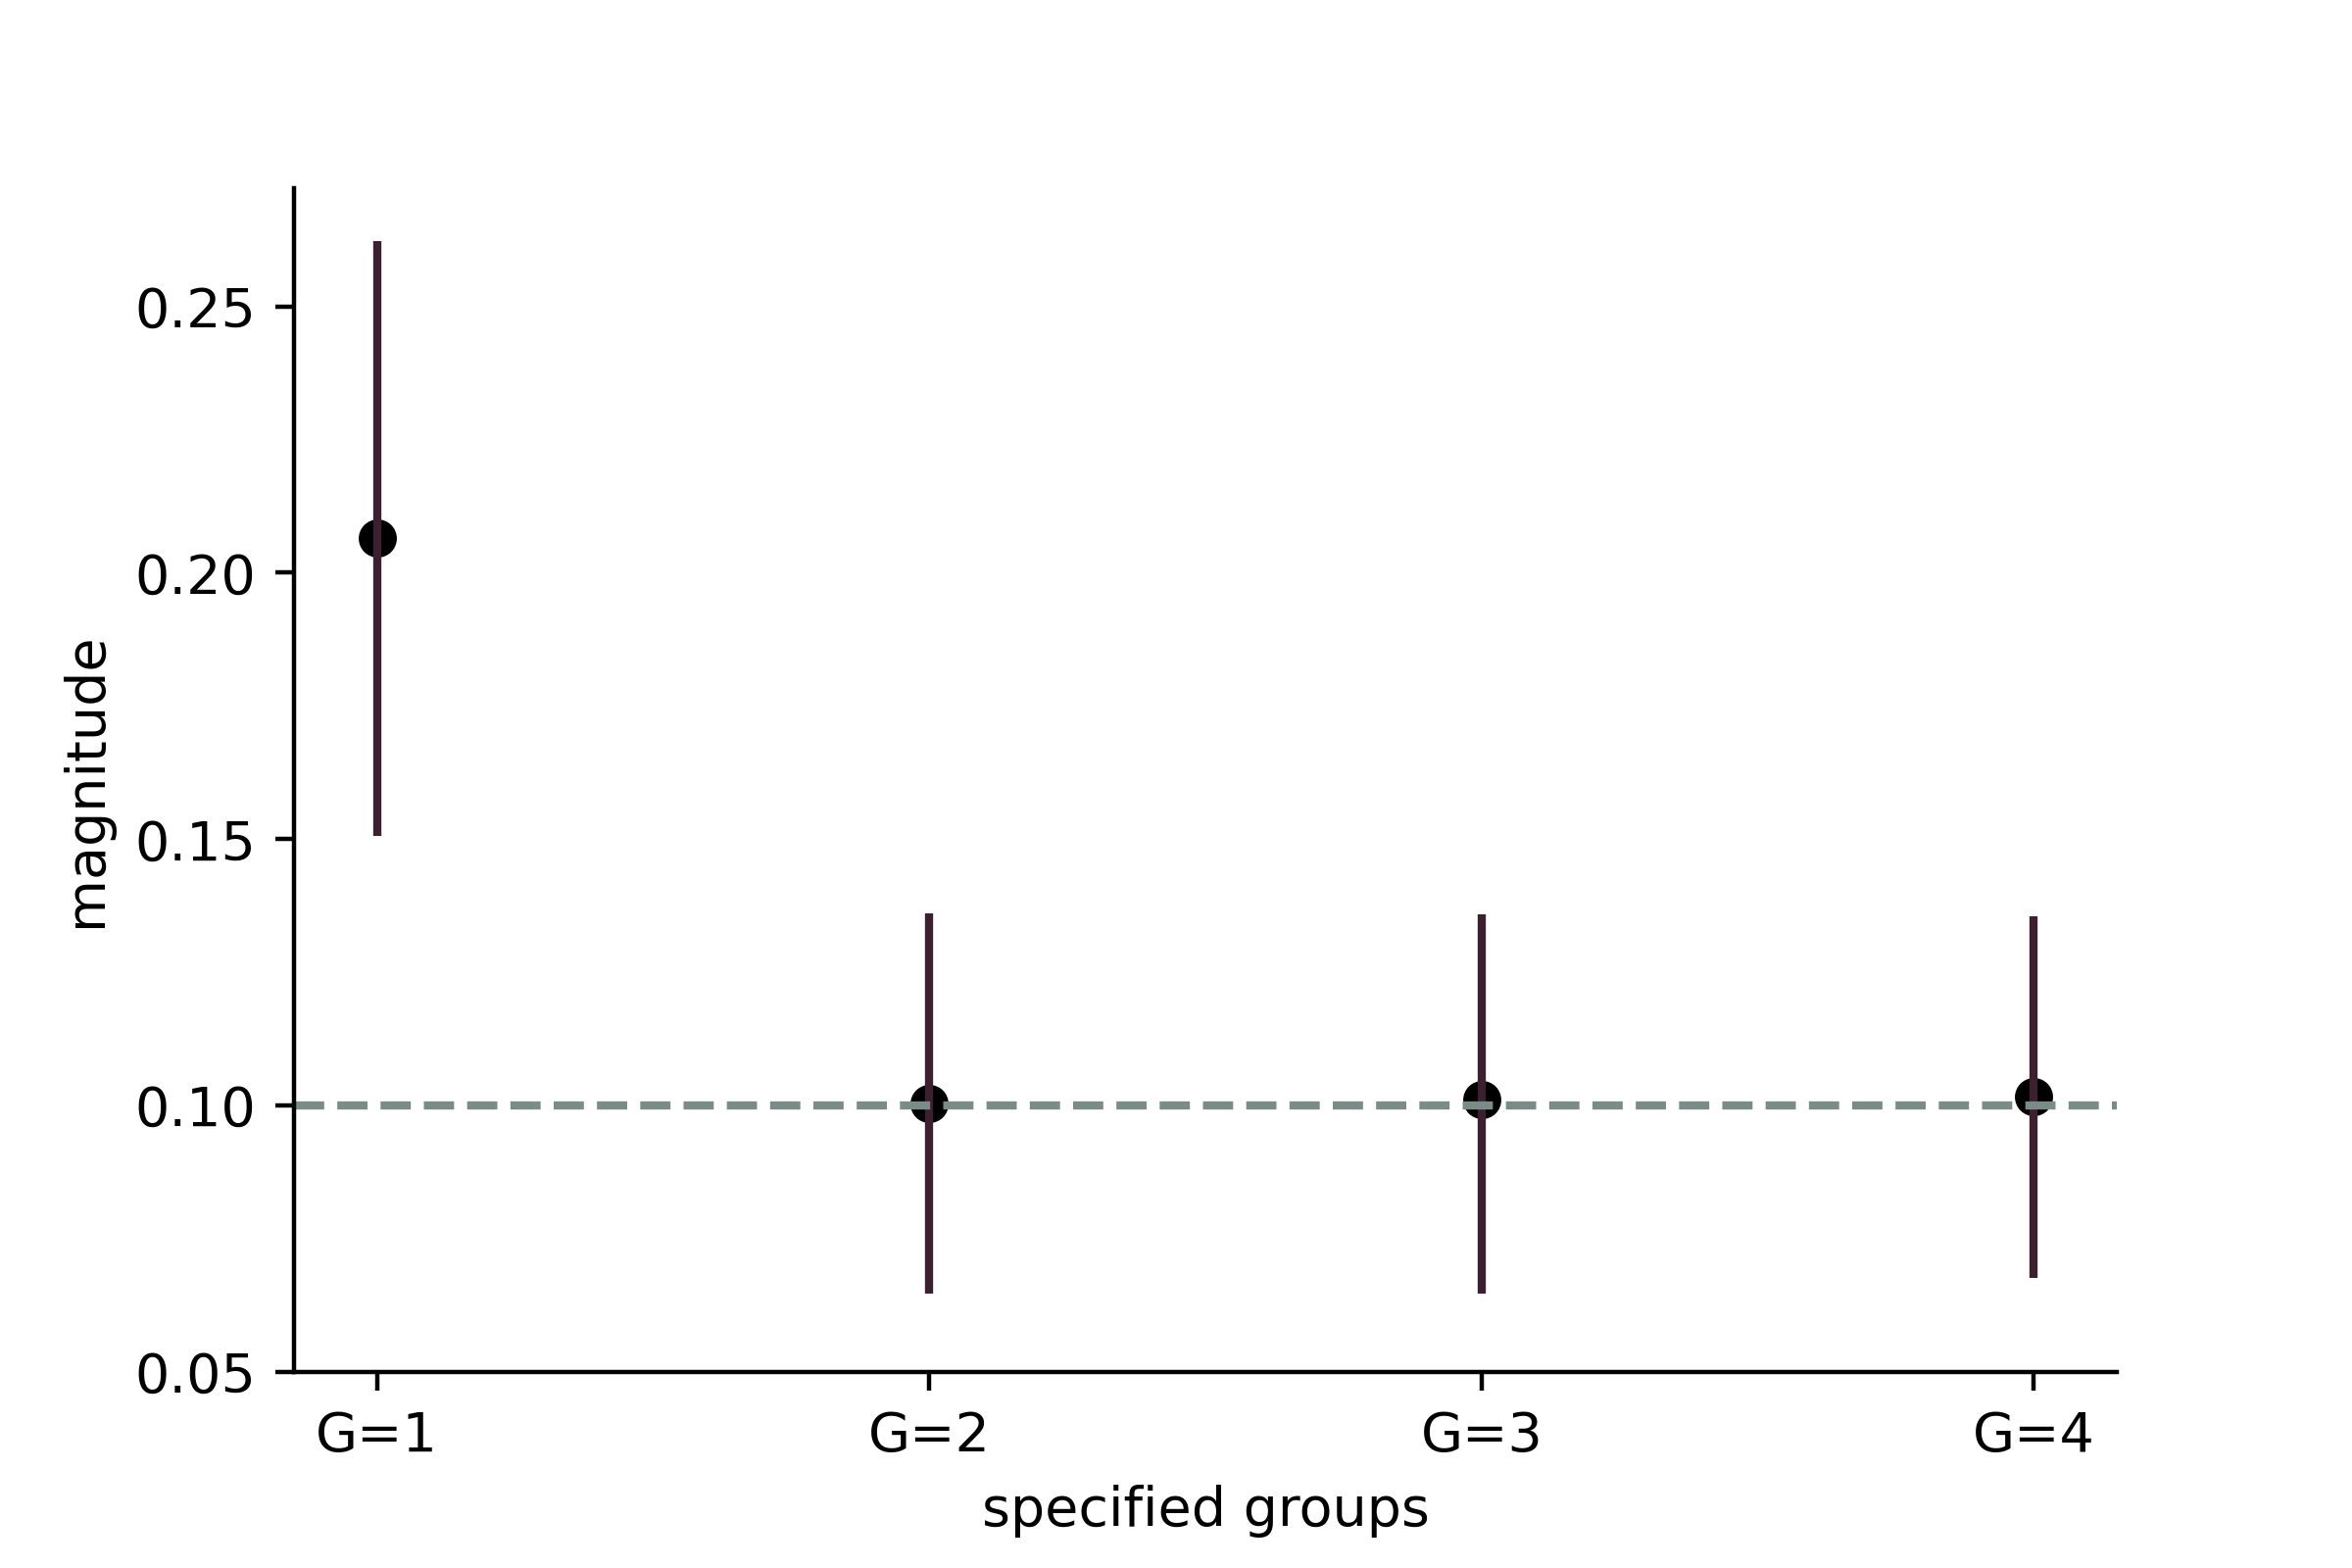
\includegraphics[scale=0.85]{figures/ciplot.png}
\caption{Expected Value and Average Confidence Intervals of $\hat{\theta}_1$ T=10, N=100.}
\label{fig:cilength}
\end{figure}
 
Finite sample properties important because it shows how the model perform in application and for inference. 


%\footnote{Model is estimated using the package in: https://github.com/FixedEffects/InteractiveFixedEffectModels.jl}

%in less precise results. Even though it does not lead to a bias and the overspecified estimator is still consistent, it has higher asymptotic variance, therefore, less efficient and less precise. It is expected that the overspecification leads to some finite sample inefficiencies. Before looking at the finite sample properties, we try to We begin by looking at the starting value of $\alpha$ for different number of groups from which we will draw heuristics.